\documentclass[conference]{IEEEtran}
%\IEEEoverridecommandlockouts
% The preceding line is only needed to identify funding in the first footnote. If that is unneeded, please comment it out.
%Template version as of 6/27/2024

\usepackage{cite}
\usepackage{amsmath,amssymb,amsfonts}
\usepackage{algorithmic}
\usepackage{graphicx}
\usepackage{textcomp}
\usepackage{xcolor}
\usepackage{hyperref}
\def\BibTeX{{\rm B\kern-.05em{\sc i\kern-.025em b}\kern-.08em
    T\kern-.1667em\lower.7ex\hbox{E}\kern-.125emX}}



\begin{document}

\title{Bart the Bartender\\
}

\author{\IEEEauthorblockN{1\textsuperscript{st} Danyal Mirza}
\IEEEauthorblockA{\textit{Department of Computer Science} \\
\textit{Uppsala University (UU)}\\
Uppsala, Sweden \\
danyal.mirza.7311@student.uu.se}
\and
\IEEEauthorblockN{2\textsuperscript{nd} Linnéa Soto Carlsson}
\IEEEauthorblockA{\textit{Department of Computer Science} \\
\textit{Uppsala University (UU)}\\
Uppsala, Sweden \\
Linnea.sotocarlsson.7666@student.uu.se}

\and
\IEEEauthorblockN{3\textsuperscript{rd} Walter Levens}
\IEEEauthorblockA{\textit{Department of Computer Science} \\
\textit{Uppsala University (UU)}\\
Uppsala, Sweden \\
walter.levens.8542@student.uu.se}
\and
\IEEEauthorblockN{4\textsuperscript{th} Adrià Irigaray Pola}
\IEEEauthorblockA{\textit{Department of Computer Science} \\
\textit{Uppsala University (UU)}\\
Uppsala, Sweden \\
email address or ORCID}

}

\maketitle

% For citations use \cite{x}, where x is defined as \bibitem{x} in references

\begin{abstract}
\textbf{Linnea + Danyal}
\end{abstract}

\begin{IEEEkeywords}
component, formatting, style, styling, insert.
\end{IEEEkeywords}

\section{Introduction}
\textbf{Linnea + Danyal}\\
The objective of the project was to design and develop "Bart", a bartender capable of reading the user's emotional state and providing drink recommendations aligning with the detected mood while engaging in a pleasant conversation. In addition, the system takes into account the individual drink preferences of the users to ensure a satisfying experience. These specific objectives were chosen in the beginning of the project, as the group members believed they were essential for creating a meaningful project connected to the course work. 
The work for this project was divided into two primary subsystems: the Perception Subsystem and the Interaction Subsystem. 

\begin{itemize}
    \item \textbf{Linnéa} and \textbf{Danyal} were responsible for developing the perception subsystem. They built a video server together with a client to connect to the interaction system. The video server is capable of detecting faces and recognizing emotions, with the help of a Random Forest (RF) machine learning model to classify mood based on facial expressions.
    
    
    \item \textbf{Adrià} and \textbf{Walter} focused on the interaction subsystem. Their work involved setting up the Furhat robot, integrating a Large Language Model (LLM) into Furhat, and designing the system to translate detected emotions and user preferences into prompts for generating personalized drink recommendations.

\end{itemize}

Teamwork within the group was collaborative and efficient, where meaningful discussions helped solving problems encountered throughout the project. The writing of the report was divided equally among the members, and each person primarily contributed to their specific area of work.
\\
\section{Methodology}
\textbf{Linnea + Danyal}
\\
This section describes the methodology and system architecture used in the project.

\subsection{Overall system design}\label{sec:overallsysdesg}
\textbf{Linnea + Danyal}


The scenario chosen for this project is as said in previous sections a bartender. The primary task of Bart, our bartender, is to analyze the customer's emotional state and offer drink recommendations based on their mood. Additionally, the system personalizes the recommendations by taking into account the customer's individual drink preferences from engaging in a pleasant conversation with the customer. This ensures a more enjoyable experience.\\The system consists of multiple parts combined into one functional, smooth system accomplishing the below stated high level goals.\\
\\
\textbf{HIGH-LEVEL GOALS:}
\\
\begin{enumerate}
    \item \textbf{Emotion Recognition:} Detect the client’s emotional state accurately based on facial expressions.
    \item \textbf{Personalized Drink Recommendations:} Suggest a drink that fits both the emotional state and the individual preferences of the client.
    \item \textbf{Engaging Conversation:} Maintain a pleasant and natural conversation with the client while offering drink recommendations.
    \item \textbf{Real-Time Interaction:} Provide real-time responses to emotions and preferences without significant delays, ensuring smooth and interactive engagement.\\
\end{enumerate}
To achieve these goals, the system consists of two sub-systems: the \textbf{perception subsystem} and the \textbf{interaction subsystem}. The perception sub-system consists of a video socket server recognizing faces combined with a machine learning model classifying emotions of recognized faces. The interaction sub-system consists of a client establishing contact with the video server, the client is integrated with Furhat, a social robot platform which is designed to enable human-like interaction through multimodal communication. Furhat have advanced speech synthesis, facial animations and gesture recognition. Furhat provides a remote API which makes it possible for us to control, design and interact with the robot over a network. Together with the client and Furhat, a Large Language Model (LLM), Gemini is integrated to the interaction subsystem to enable a response to the user speech input.\\
\subsection{User perception sub-system}
\textbf{Linnea + Danyal}
\subsubsection{Server design}\label{sec:serverdesign}
To allow emotion detection, a video server had to be created that captured video of user interacting with Furhat. The video server begins with establishing a socket connection with the Furhat client to allow communication between the two subsystems. The server then begins capturing video and for each current frame uses py-feat to detect faces and AU-values are then sent to our trained machine learning model to predict emotion. A message containing the following information is then sent to the client via the socket connections:
\begin{itemize}
    \item Number of faces detected
    \item Values representing location of the face
    \item Predicted emotion
\end{itemize}
\subsubsection{Machine Learning Design}
The random forest machine learning model for emotion detection was developed through several steps with the goal to optimize performance. Before deciding on random forests as the primary model, several other machine learning approaches were explored, including Support Vector Machines (SVM), boosting, and neural networks. This process is discussed more thoroughly in the discussion headline of this report.\\ The first step in building the model was identifying and preparing a dataset suitable for the emotion detection task.

We decided to start with the dataset used for Assignment 2 but when used in training and validating the accuracy value would vary a lot. This led us to believe that the low amount of data would make it easy to under-fit or over-fit. To solve this, we decided to expand our dataset from 1,100 entries to 4,300 entries. To make the system a bit more robust we decided to also add data from real faces, we did this because we considered the AI-generated images to have exaggerated proportions in some cases and it may not reflect reality as well. The other dataset used was extracted from a Kaggle Facial Expression Recognition Challenge \cite{kaggle} associated with "ICML 2013 Workshop on Representation Learning". The dataset seemed specially good for this application as its purpose was emotion recognition.
We still decided to include the first dataset because the more expressive emotions are also useful in a bar scenario later in the night.

For extracting AUs no preprocessing was deemed necessary but we did need some postprocessing, this was
due to the images being extracted from the internet; some faces were obscured or rotated to the point
of being unrecognizable by the algorithm. Having a very large amount of entries, we decided to delete any entry with missing values so that them
machine learning wasn't using "corrupted" data. In the end we had 4300+ images with extracted AU values combined from 2 datasets.


Once the dataset was prepared, it was split into an 80\% training set and a 20\% test set using stratified sampling to keep the original class distribution. An initial analysis of the class distribution revealed significant imbalances in the emotion categories:
\begin{itemize}
    \item Neutral: 20.97\%
	\item Happy: 20.95\%
	\item Surprise: 16.86\%
	\item Sad: 11.95\%
	\item Fear: 11.74\%
	\item Angry: 10.42\%
	\item Disgust: 7.11\%
\end{itemize}	
To address this imbalance, the Synthetic Minority Oversampling Technique (SMOTE) was applied to the training set, resulting in a more even distribution across classes. SMOTE is a technique to balance uneven distribution of classes by synthesizing samples in minority classes. The selection of synthesized value is decided through k-nearest neighbors within the class in question. This was done to avoid overfitting and bias in the training dataset.  
\\Following this, a baseline random forest model was trained.
This baseline model was then optimized with the help of a thorough grid search in the process of finding a better accuracy and stability. A random search was initially included in the process, which later was removed from the code to make it more concise, as its performance did not match that of the grid search using GridSearchCV.
\\
The hyperparameters tuned during this process included:
\begin{itemize}
    \item Number of estimators (n\_estimators)
	\item Maximum tree depth (max\_depth)
	\item Minimum samples for node splits and leaves (min\_samples\_split, min\_samples\_leaf)
	\item Number of features considered for splitting (max\_features)
	\item Use of bootstrapping (bootstrap)
\end{itemize}	
    
The optimization process had 5-fold cross-validation.
Model performance was assessed using a classification report that included precision, recall, F1-score, and accuracy.
\\The above mentioned process was repeated but this time without the SMOTE to compare the performances of the resulting models. This process proved the model without the SMOTE to be the best performing model. This model had the Best Hyperparameters: 
\texttt{(bootstrap: True, max\_depth: 30, max\_features: sqrt, min\_samples\_leaf: 1, min\_samples\_split: 2, n\_estimators: 100)}. The model has the accuracy of 46.46\%. To asses the generalizability of the model a out-of-bag (OOB) score was also calculated. The model has an OOB-score of 0.45 which is close to the accuracy score of the model, indicating that the model is good at generalizing to unseen data\cite{OOB}.\\

\subsection{Interaction sub-system} %Walter + Danyal
This section discusses the second subsystem of Bart the bartender, which handles the interaction with the user. 
It goes over the high-level design and its implementation. 
Afterwards it evaluates the obtained results.

\subsubsection{Design}
The interaction sub-system in this project consists of the virtual Furhat, as described in section \ref{sec:overallsysdesg}, Gemini and a connection to the video server, which has been described in section \ref{sec:serverdesign}.
Furhat is used as the interface between the system and the user and Gemini is used to generate a response to the input of the user.
The response is based on what the user says and what emotion is detected in the face of the user at the beginning of the conversation.
This response is then sent to Furhat so that it can reply to the user.
This process is repeated until the right drink is found for the user.

\subsubsection{Considering a group of people}
When there is a group of people, the bartender considers the person who is closest to Furhat which matches the logic of how a bartender would work. If there is a queue of people waiting to order, it does not make sense to interact with a person who is not first in the queue. The logic of deciding who is closest to Furhat is decided by who has the biggest face box. If there are two people equally close Furhat, the choice of who to consider becomes undecidable and both faces may be considered. However, we deem this to be a reasonable interaction.

\subsubsection{Implementation}
The typical flow of this subsystem is as follows: 
A connection is set up between this subsystem and the video server that was described in the previous section.
Once this connection is set up, Bart greets the user and asks what kind of cocktail the user wants.
From this moment, the subsystem gathers the detected emotions of the user, until the user is done with speaking.
From these emotions, we determine the dominant emotion of the user.
When the user finishes their reply to Bart, we combine the dominant emotion with the reply of the user and send it to Gemini.
Gemini is a LLM that is instructed to act like a bartender that recommends cocktails that fit the mood of the customer.
We decided to use Gemini because it is free for people with a google account up to a rate limit.
Our application does not use up a lot of tokens, so we should not reach this rate limit.
Once Gemini has generated a response, it is forwarded to Bart.
Then, Bart is instructed to say the response.
After Bart is done with talking, it listens again for input of the user. 
The input of the user is again combined with the dominant emotion and sent to Gemini.
This cycle continues until the user decides on a cocktail.
After this the whole cycle repeats from the beginning, assuming there is a new customer.

% The interaction sub-system mostly resides in a file called \textit{client\_receive.py}.
% This file first sets up the connection to the video server and after that it listens for messages from the server.
% In our case, messages from the server contain information about the faces in the frame.
% This includes emotion and postion of the face.
% The system decides at the beginning of the conversation with the user what the most dominant emotion of the user is.
% It does this by gathering all detected emotions until the user gives their first input.
% While \textit{client\_receive.py} listens to messages from the server, it also listening for input of the user.
% If the user is done with talking, their message is combined with most dominant emotion .
% This prompt is then given to Gemini, which creates a fitting response.
% We chose Gemini for this project because it is free to use with a Google account and it has a rate limit that we will most likely not reach.
% To make sure Gemini generates a fitting response, it is given a system instruction that precisely describes its role as a bartender.
% The response that is generated by Gemini is then forwarded to furhat so it can reply to the input of the user.
% After this is done, furhat starts listening to the user again and this process is repeated.
% Once Bart finds a fitting cocktail it says `Here you go' and afterwards listens to input from a new user.

\subsubsection{Result}
In the project proposal, we described several objectives that we expect our bartender to fullfill.
We can test our product by confirming it adheres to the set objectives.

One of the objectives is that our product gives recommendations to the user, based on the user's emotional state.
We add the mood of the user to the prompt that we send to Gemini.
Because of this, Gemini will take both the emotion of the user as well as the user's speech into account when generating a response.

Another objective is that Bart should take the user's preferences into account. 
We achieve this by letting Gemini generate questions that explores the needs and preferences of the user.
Gemini incorporates current and previous answers of this user into the recommendation.

The last objective is that the conversation with the system should be pleasant.
This is a more subjective goal, but we try to make the conversation as pleasant as possible by continuously adjusting the prompts given to Gemini.
By doing this, we hope to make the conversation as pleasant as possible.

% - works well in general, it finds a cocktail based on the input of the user relatively quickly
% objectives from specification:
% - come up with recommendations based on emotional state -> reflects on current emotional state of user
% - take the preferences of the client into account -> automatically happens due to prompting of llm
% - make sure the conversation is pleasant -> subjective, hard to tell (conduct interviews etc.)

\section{General Discussion}
Adria\\

\subsection{Overall Pipeline}
\begin{figure}[!h]
    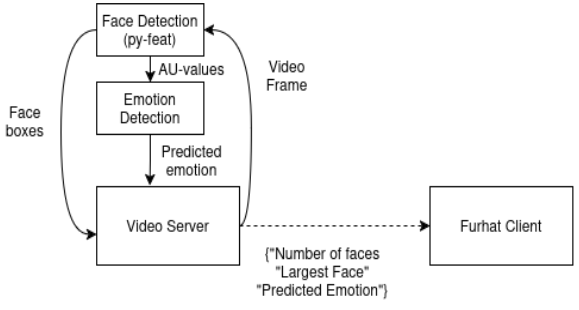
\includegraphics[width=\linewidth]{pipeline.png}
    \caption{How our system works.}
    \label{fig:pipeline}
  \end{figure}

Our system works by separating the video server from the Furhat client. The video server (Seen in Fig.1) constantly captures an image,
gets the face box and the AU values, predicts and emotion from the AUs and sends a message with the number of faces, the emotions found, and which emotion corresponds to the largest face.

The Furhat client then accumulates the emotions until the user responds to the initial question: "Hello, what Cocktail can I get for you?".
It then uses the most displayed emotion to indicate the LLM how to act alongside the user input.

Once the user decides a drink Bart says "Here you go!" as an indication that the conversation is finished and the accumulated values are reset to 0 so that
it can start attending the next client.
\subsection{Challenges}
We had initial issues training due to the low ammount of data. However, once this was solved training progressed more steadily.


The path to selecting the Random Forest model involved several steps and a lot of experimentation with different approaches. First we explored building our own neural networks, specifically multilayer feedforward neural networks using a gradient backpropagation algorithm. We tested various architectures to improve the accuracy of emotion classification. However, this approach was highly time-consuming in terms of training and optimizing the networks. The results were also often unstable, and fine-tuning the neural network models required more resources and time than the scope of our project and expertise would allow.


Next we found a pre-trained model for facial recognition from a competition on Kaggle\cite{kaggle}. We experimented with replication of the model adjusted to our own expertise. This did approach did however not lead to desired outcomes. Even though pre-trained models were allowed, we decided against using them unmodified because we wanted the work to reflect our own understanding and contributions. Given that the machine learning model was a major component of the project, relying on someone else’s model did not feel right.

Due to this we shifted our focus to other machine learning methods. We experimented with Support Vector Machines (SVM), Boosting models, and finally, Random Forest models. After thorough testing, we found that the Random Forest model had best balance of accuracy and stability even though we would preferably have wanted to have more time to improve its results, this was however not possible considering our work load combined with other courses. The RF-model performance was consistent across test runs, and due to this it ultimately became the chosen model for our system.
\subsection{Use of ChatGPT and other tools}

ChatGPT has been used to assist in resolving error messages in the code and to discuss different ways to optimize machine learning techniques. The information provided by ChatGPT has been cross-verified with other sources, including GeeksforGeeks and the official Python documentation for specific packages. Using ChatGPT helped streamline our workflow by providing quick solutions to technical challenges and offering alternative approaches to improve model performance. Additionally, it saved significant time during debugging and allowed us to focus on implementing and testing new ideas, ultimately enhancing our understanding of machine learning concepts.

AI has also been used as a proof reader of our project report and gave us valuable help with formulation of sentences and handling of grammatical errors. This significantly improved the flow and readability of our report. 

\subsection{Ethical Issues}
Due to the nature of our project the main ethical issues that we could encounter would be related to the LLM system.
We don't use our own model so many things are left for Gemini and its API. For example, we do not apply any filters to the LLM's response.
This means that if the user is rude to the AI there's nothing stopping it from insulting back or being generally unpleasant. Right now there's nothing stopping
The AI from recommending things that are not available or other similar issues. We are also not aware of how secure is the communication between the robot
and the LLM servers so there is a possibility of personal information being leaked.

We are less concerned about information storage on our end, the user's AUs are only stored in RAM until the emotion is detected and conversations are not stored.
The only information we store is the emotional state of the user but that gets reset after every drink.

The other possible issue found is the replacement of bartenders. With the project so far this is unlikely,
our system doesn't prepare the cocktails so a human element is still needed (unless the system works like a soda machine but
it wouldn't be pleasant). Even if it were not needed Bart has a limited capacity to give conversation about recent events so it would be lonely if not accompanied by a flesh and blood bartender.




\section*{Conclusion}
Bart tool is very useful for busy days and maybe more socially awkward costumers. Before implementation on a buisness additional information like
the current menu, which are the house special drinks, information about the restaurant's facilities and other similar information should be added
to the system so that it can answer correctly customer questions. More training would be necessary as Bart only picks up on expressive faces
but doesn't quite work with more muted facial expressions. 

\begin{thebibliography}{00}
\bibitem{kaggle} Dumitru , ``Kaggle'' Available:  \href{https://www.kaggle.com/c/challenges-in-representation-learning-facial-expression-recognition-challenge/overview}{https://www.kaggle.com/}. Contest associated with the ICML 2013 Workshop on Representation Learning.

\bibitem{OOB} H. L. Smith, P. J. Biggs, N. P. French, A. N. H. Smith, J. C. Marshall, ``Out of (the) bag—encoding categorical predictors impacts out-of-bag samples,'' November 18, 2024. \href{https://doi.org/10.7717/peerj-cs.2445}{DOI: 10.7717/peerj-cs.2445}.


\end{thebibliography}

\end{document}
